\documentclass[12pt]{article}
\usepackage[utf8]{inputenc}
\usepackage[T2A]{fontenc}
\usepackage{libertine}
\usepackage[a4paper, left = 2.5cm,right = 2.5cm,top = 2.5cm,bottom = 3cm]{geometry}
\usepackage[english,russian]{babel}
\usepackage{amsmath}
\usepackage{amssymb}
\usepackage{amsfonts}
\usepackage[final]{graphicx}
\usepackage[linktocpage=true, colorlinks=true, linkcolor = blue, citecolor = red]{hyperref}
\usepackage{cmap}
\usepackage{xfrac}
%\usepackage[titletoc]{appendix}
\usepackage{pgfplots}
\usepackage{cite}
\newcommand{\eprint}{}

%\linespread{1.2}

\newcommand{\bq}{\begin{equation}}
\newcommand{\eq}{\end{equation}}

\usepackage{tikz}
%%%%%%%%

\begin{document}

\title{Explisit isometric embeddings of collapsing black hole}
\author{
A.~D.~Kapustin\thanks{E-mail: sashakapusta96@gmail.com},
S.~A.~Paston\thanks{E-mail: pastonsergey@gmail.com}\\
{\it Saint Petersburg State University, Saint Petersburg, Russia}
}
\date{\vskip 15mm}
\maketitle

\begin{abstract}
В этой работе ищутся явные вложения наименьшей размерности для метрики коллапсирующего сферически симметричного облака пылевидной материи, образующего Шварцшильдовскую черную дыру. В работе рассматриваются два подхода, в одном из которых находится глобальное семимерное вложение с изломом, а в другом локальное семимерное, также содержащее излом. Однако для частного случая во втором подходе удается найти гладкое шестимерное вложение, покрывающее все области многообразия.
\end{abstract}

\clearpage

\section{Введение}
Как известно (см., например, \cite{goenner}), любое (псевдо)риманово многообразие размерности $d$ может быть \emph{изометрически} вложено в \emph{плоское} объемлющее пространство размерности $N \geqslant d(d+1)/2$ как минимум локально.
В результате многообразие можно описывать функцией вложения $y^a(x^\mu)$, а метрику считать \emph{индуцированной}
\bq\label{s1}
	g_{\mu \nu} = (\partial_{\mu} y^a) (\partial_{\nu} y^b) \eta_{ab},
\eq
где $\eta_{ab}$ -- плоская метрика объемлющего пространства; здесь и далее $\mu,\nu=0,...,d-1$; $a,b=1,...,N$.
Такой способ описания многообразия может оказаться наглядным и полезным для изучения его структуры, однако он требует отыскания явного вида функции вложения для заданной метрики $g_{\mu\nu}$, т.е. решения дифференциального уравнения \eqref{s1} относительно $y^a$. Изучение структуры многообразия особенно актуально в отношении черных дыр, так как соответствующие им многообразия обычно имеют нетривиальную структуру.
 
Для невращающейся незаряженной черной дыры, соответствующей метрике Шварцшильда, первое явное вложение было построено еще в 1921 году \cite{kasner3},
однако оно (равно как и вложение \cite{fudjitani}) применимо только вне горизонта, поэтому для изучения структуры многообразия непригодно.
Наиболее полезное для такой цели вложение было предложено в 1959 году в работе \cite{frons}, оно, оставаясь везде гладким, применимо
как вне, так и внутри горизонта, причем соответствует максимальному аналитическому расширению решения Шварцшильда,
которое включает в себя две области вне горизонта (две вселенные) и две области под горизонтом, соответствующие черной и белой дырам.
Кроме перечисленных, известно еще три так называемых "минимальных"{} (т.е. соответствующих минимально возможной размерности
объемлющего пространства, в данном случае равной 6 \cite{kasner2}) вложения \cite{davidson,statja27} метрики Шварцшильда, которые покрывают
половину упомянутого максимального аналитического расширения -- например, совокупность области вне горизонта и области под горизонтом, соответствующей черной дыре,
см. подробности в \cite{statja27}.
Отметим, что только именно эти две области имеют место, если вместо максимального аналитического расширения, соответствующего \emph{вечной}
черной дыре, рассматривать риманово пространство, соответствующее черной дыре, возникающей в результате коллапса.

Задача поиска минимальных \emph{глобальных} (т.е. гладких при всех значениях радиуса, включая точки горизонтов)
вложений для невращающейся заряженной черной дыры Райсснера-Нордстрема рассматривалась в работе \cite{statja30}.
Было построено три варианта вложения, которые могут использоваться как для случая nonextremal charged black hole,
так и для случаев extremal and hyperextremal one. Обобщение на случай присутствия космологической постоянной изучалось в  работе \cite{statja40}.
Для физически более интересного случая вращающейся черной дыры Керра, равно как и для его обобщения -- заряженной вращающейся черной дыры Керра-Ньюмена,
задача построения явных вложений оказывается гораздо более сложной из-за более маленькой группы симметрии задачи.
Известны только записанные в неявном виде (в виде двух дифференциальных уравнений на две неизвестные компоненты функции вложения)
локальные вложения в 9-мерное объемлющее пространство \cite{kuzeev} и \cite{kuzeevRN} (для метрик Керра и Керра-Ньюмена соответственно)
и 14-мерное вложение метрики Керра, предложенное в работе \cite{gr-qc/0503079}.

Нахождение явных вложений для физически интересных решений теории гравитации может быть полезным
еще и с точки зрения изучения описания гравитации в рамках теории вложения -- гравитации Редже-Тейтельбойма, впервые предложенной в работе \cite{regge}.
В рамках этого подхода именно функция вложения $y^a(x)$ является независимой переменной вместо метрики,
которая выражается формулой \eqref{s1}.
После \cite{regge} возможность использования идеи изометрического вложения для описания гравитации, в том числе и в связи с ее квантованием,
неоднократно обсуждались в работах разных авторов, см., например,
работы \cite{deser,pavsic85let,tapia,davkar,statja18,rojas09,statja25,faddeev,statja51}.
Явные вложения римановых многообразий с горизонтами также используются при анализе связи между излучением Хокинга
и излучением Унру, соответствующим движению наблюдателя в объемлющем пространстве \cite{deserlev98,deserlev99,statja36}.
Подробный список литературы, связанной с теорией вложения и смежными с ней вопросами, может быть найден в обзоре \cite{tapiaob}.

Сложность задачи построения явных вложений для произвольного четырехмерного пространства-времени связана с тем, что
необходимо решать систему $10$ дифференциальных уравнений  в частных производных \eqref{s1} относительно функции вложения $y^a(x^\mu)$,
зависящей от $4$ координат $x^\mu$.  
Задача упрощается, если у многообразия присутствуют дополнительные симметрии.
Их наличие позволяет использовать конструктивный метод построения явных вложений \cite{statja27}, который при
достаточно большой симметрии может свести задачу к решению системы ОДУ.
Именно так происходит для метрик Шварцшильда и Райсснера-Нордстрема, обладающих симметрий $SO(3)\times T^1$, где $T^1$ обозначает трансляционную симметрию
относительно сдвигов времени. Аналогична ситуация (см.~\cite{statja29}) и для космологических решений --
для метрик всех трех моделей FRW, обладающих симметриями: $SO(4)$ для закрытой модели, $SO(1,3)$ для открытой модели
и группой движений трехмерной плоскости для пространственно-плоской модели.

Самым, наверное,  интересным с физической точки зрения вариантом черной дыры является черная дыра, возникающая в результате коллапса,
при котором облако материи сжимается, образуя черную дыру динамически. В таком процессе происходит образование горизонта
и поэтому особенно интересным становится изучение структуры соответствующего многообразия, а значит актуальной становится
задача постоения явного вложения для этого случая.
Даже если пренебречь вращением, т.е. считать, что вне области нахождения материи метрика определяется
решением Шварцшильда, то построить явное вложение для соответствующей этому случаю метрики оказывается
сложной задачей. Именно построению таких вложений посвящена настоящая работа, до сих пор они не были известны.
Для упрощения задачи мы берем простейший вариант поведения коллапсирующей материи, рассматривая коллапс
состоящего из пылевидной материи однородного шара. 

Группой симметрии этой задачи является $SO(3)$ и эта симметрия оказывается недостаточно богатой, для сведения задачи
к решению системы ОДУ в рамках метода \cite{statja27}. Однако, если рассматрвать многообразие как совокупность двух частей --
содержащей материю (сжимающийся пылевидный шар) и не содержащей ее (область вне этого шара), то для каждой
из частей симметрия оказывается выше. Для области вне шара метрика согласно известной теореме Биркгофа
представляет собой метрику Шварцшильда, а значит обладает симметрией $SO(3)\times T^1$ и мы для нее знаем
упомянутый выше ряд вложений. Для области же внутри шара, метрика соответствует одной из моделей FRW, см., например, \cite{landavshic2},
а значит, тоже обладает расширенной симметрией соответствующего типа и вложения такой метрики известны.
Такая ситуация позволяет найти вложения для всего многообразия путем сшивки модифицированных подходящим образом
известных вложений его частей.

В разделе 2 рассматриваются две системы координат, используемые в работе. В разделе 3 рассматривается случай, в котором удается построить вложение коллапса, не прибегая к сшивке известных вложений. В разделе 4 рассматривается построение вложения, основанное на сшивке вложений для геометрии Шварцшильда и геометрии FRW, и частный случай, в котором удается построить вложение коллапса минимальной размерности.

\section{Используемые координатные системы}
Для построение вложения сперва необходимо найти метрику, являющуюся решением уравнений Эйнштейна (\ref{G=T}) с ТЭИ, соответствующему выбраному типу материи и ее распределению.
\begin{equation}
\label{G=T}
	G_{\mu \nu} = \varkappa T_{\mu \nu}.
\end{equation}
Для пылевидной материи ТЭИ выглядит наиболее просто, если использовать систему синхронных сопутствующих координат, а, в силу сферической симметрии, в качестве двух пространственных координат выбрать углы $\theta$ и $\varphi$. Оставшуюся времениподобную координату обозначим $\tau$, а пространственноподобную --- $\chi$. 

Решение уравнения (\ref{G=T}) можно искать в виде диагональной метрики. Для произвольного распределения материи оно имеет вид
\bq
\label{metric}
	d s^2 = d \tau^2 - \frac{(r'(\tau, \chi))^2}{1+f(\chi)} d\chi^2 - r^2(\tau, \chi) d \Omega,
\eq
где функция $r(\tau, \chi)$ определяется одним из трех способов
\bq
\label{v123}
	r(\tau, \chi) = \left\{
	\begin{matrix}
	\frac{F(\chi)}{2 f(\chi)} H \left( \frac{2(f(\chi))^{\sfrac{3}{2}} }{F(\chi)}(\tau_0(\chi)-\tau)  \right) , \ \ \ \ f(\chi) > 0,\\
	\left( \frac{9F(\chi)}{4} \right)^{\sfrac{1}{3}} \left[ \tau_0(\chi)- \tau \right]^{\sfrac{2}{3}}, \ \ \ \ f(\chi) = 0, \\
	- \frac{F(\chi)}{2 f(\chi)} E \left( \frac{2(-f(\chi))^{\sfrac{3}{2}} }{F(\chi)}(\tau_0(\chi)-\tau) \right), \ \ \ \ f(\chi) < 0.  
	\end{matrix} \right.
\eq
Функции $E(x)$ и $H(x)$  служат для обращения параметрических зависимостей
\bq
	\begin{array}{c}
	E = 1 - \cos{\eta}, \\
	x = \eta - \sin{\eta},
	\end{array} \ \ \ \ \ \ \ \
	\begin{array}{c}
	H = \ch{\eta}-1, \\
	x = \sh{\eta} - \eta,
	\end{array}
\eq
а функции $F(\chi), f(\chi)$ и $\tau_0(\chi)$ задают распределение плотности материи и начальные скорости. Более подробный вывод можно найти в \cite{landavshic2}.

Если потребовать однородности распределения материи в начальный момент, то пространство внутри коллапсирующего шара будет описываться геометрией открытой, пространственно-плоской или закрытой модели Фридмана соответственно выбору первого, второго или третьего способа определения $r(\tau, \chi)$ в формуле (\ref{v123}). Внешнее к шару пространство, согласно теореме Биркгофа, во всех случаях описывается геометрией Шварцшильда. Метрика (\ref{metric}) в случае однородной плотности материи будет иметь координатную особенность в виде скачка на границе шара, которую можно устранить переходом к координатам $(\tau, r, \theta, \varphi)$, что будет использовано в разделе 3. 

Произведем описанную замену координат. Тогда метрика общего вида (\ref{metric}) перейдет в 
\bq
	d s^2 = \left( 1- \frac{\dot{r}^2}{1+f(\chi)}\right) d \tau^2 + 2\frac{\dot{r}}{1+f(\chi)}dr d\tau - \frac{dr^2}{1+f(\chi)} - r^2 d\Omega.
\eq
Если теперь выбрать $f(\chi)=0$, то $r(\tau, \chi)$ выразится через элементарные функции и можно вычислить $\dot{r} = \frac{\partial r(\tau, \chi)}{\partial \tau}$. После всех преобразований метрика примет вид
\bq
\label{metric2}
	d s^2 = \left(1-\frac{4F(\tau, r)}{9 r} \right)d\tau^2 - 2 \frac{3}{2}\sqrt{\frac{F(\tau, r)}{r}}dr d\tau  - dr^2 - r^2 d\Omega.
\eq

В этих координатах метрика непрерывна всилу необходимой непрерывности фуункции $F(\tau, r)$.

\section{Построение вложения без сшивания}

Продвинуться на пути построения вложения для метрики (\ref{metric2}) удается если потребовать однородной плотности. Чтобы метрика (\ref{metric2}) отвечала однородной плотности материи в шаре, следует выбрать
\bq
	F(\tau, r) = \min{ \left( \frac{r^3}{(1-\tau)^2}, F_0 \right) }.
\eq
Тогда видно, что метрика оказывается непрерывной, однако не всюду дифференцируемой функцией.

\begin{figure}[h!]
	\centering
	\begin{tikzpicture}[scale=0.75]
		\draw[->] (-5, 0) -- (5, 0)node[below]{$u$};
		\draw[->] (0, -5) -- (0, 5)node[left]{$v$};
		%%
		\draw[->] (4.5, 0.5) -- (5.5, 0.5)node[midway,above]{$r \to \infty$};
		%%
		\begin{scope}
		\clip (7.5, 6) -- (5, 6) -- (0.6, 2.8) .. controls (1, 1) and (1, 0) .. (5, -3) -- (5, -6) -- (7.5, -6) -- cycle;
		\draw[thick, dashed] (-5, -5) -- (5, 5)node[above right]{$r = R$};
		\draw[thick, dashed] (-5, 5) -- (5, -5);
		%%
		\draw (5, 4.9) .. controls (0, 0) and (0, -0) .. (5, -4.9);
		\draw (5, 4.7) .. controls (1.5, 1) and (1.5, -1) .. (5, -4.7);
		\draw (5, 4.5)node[below right]{$r=const$} .. controls (3, 1.5) and (3, -1.5) .. (5, -4.5);
		%%
		\draw (-5, 4.9) .. controls (0, 0) and (0, -0) .. (-5, -4.9);
		\draw (-5, 4.7) .. controls (-1.5, 1) and (-1.5, -1) .. (-5, -4.7);
		\draw (-5, 4.5) .. controls (-3, 1.5) and (-3, -1.5) .. (-5, -4.5);
		%%
		\draw (4.9, 5) .. controls (0, 0) and (0, 0) .. (-4.9, 5);
		\draw (4.8, 5) .. controls (1, 1) and (-1, 1) .. (-4.8, 5);
		\draw[ultra thick] (4.7, 5) .. controls (2, 2) and (-2, 2) .. (-4.7, 5);
		%%
		\draw (4.9, -5) .. controls (0, 0) and (0, 0) .. (-4.9, -5);
		\draw (4.8, -5) .. controls (1, -1) and (-1, -1) .. (-4.8, -5);
		\draw[ultra thick] (4.7, -5) .. controls (2, -2) and (-2, -2) .. (-4.7, -5);
		\draw (0, -3)node[below right]{$r = 0$};
		%%
		\end{scope}
		\draw (0, 3)node[above right]{$r = 0$};
		\draw[blue, very thick] (5, -3) .. controls (1, 0) and (1, 1) .. (0.6, 2.8);
	\end{tikzpicture}
	\caption{\label{infkrusk}The Kruskal diagram for matter collapsing from infinity.}
\end{figure} 

Можно представить область пространства, соответствующую константе $F_0$, на диаграмме Крускала, представленной на Рис. \ref{infkrusk}. Она ограничена мировой линией частицы, лежащей на границе сферы. Для этого случая характерно то, что коллапс происходит с бесконечности, в отличие от второго подхода. Оставшаяся часть многообразия описывается метрикой Фридмана и может быть восстановлена с помощью построеного вложения.

Как уже упоминалось в разделе 2, выбор $f(\chi)=0$ соответствует тому, что часть пространства, содержащая материю описывается пространственно-плоской моделью Фридмана.

\subsection{Построение вложения для полученной метрики}

Если ввести переменные $t = (1-\tau)^{\sfrac{2}{3}}$ и $p = \frac{r^3}{(1-\tau)^{\sfrac{4}{3}}}$, метрика примет вид
\bq
	d s^2 = \left(\alpha t +f(p) \right) dt^2 + h(p) t \ dp dt - \left(dr(t,p)\right)^2 - r^2(t,p) d \Omega,
\eq
где 
\[
\alpha = \frac{9}{4},\ \ \ \  f(p) = 2 F(p)^{\sfrac{1}{2}} p^{\sfrac{1}{6}} - F(p) p^{-\sfrac{1}{3}}, \ \ \ \  h(p) = \frac{2F(p)^{\sfrac{1}{2}}}{3p^{\sfrac{5}{6}}}.
\]

Если в качестве трех функций вложния выбрать блок $(r \cos{\theta},r \sin{\theta}\cos{\varphi},r \sin{\theta}\sin{\varphi})$, то останется вложить метрику
\bq
	d s^2 = \left(\alpha t +f(p) \right) dt^2 + h(p) t \ dp dt.
\eq
Видно, что ее компоненты являются полиномами по переменной $t$. Тогда можно искать решение уравнений вложения также в виде полиномов. Удобнее всего это сделать в светоподобных координатах объемлющего пространства. Решение представимо в виде
\begin{align}
	y^{+} &= t^3 - \frac{\alpha}{4}t^2-\frac{f(p)}{2}t, \\
	y^1 &= \sqrt{\frac{3}{2}}t^2 + \frac{1}{\sqrt{6}}\int h(p)dp - \frac{1}{2\sqrt{6}}f(p), \\
	y^{-} &= t, \\
	y^{3} &= \frac{1}{\sqrt{6}}\int h(p)dp - \frac{1}{2\sqrt{6}}f(p).
\end{align}
Чтобы получить полный набор функций вложения нужно дописать блок
\begin{align}
	y^4 &= p^{\sfrac{1}{3}}t \cos{\theta}, \\
	y^5 &= p^{\sfrac{1}{3}}t \sin{\theta} \cos{\varphi}, \\
	y^6 &= p^{\sfrac{1}{3}}t\sin{\theta} \sin{\varphi}.
\end{align}

Итого, если вернуться к более естественным переменным, получится набор функций вложения
\begin{align}
	y^{+} &= (\tau')^2 - \frac{\alpha}{4}(\tau')^{\sfrac{4}{3}}-\frac{f\left(\frac{r^3}{(\tau')^2}\right)}{2}(\tau')^{\sfrac{2}{3}}, \\
	y^1 &= \sqrt{\frac{3}{2}}(\tau')^{\sfrac{4}{3}} + \frac{1}{\sqrt{6}}\int \limits_C^{\frac{r^3}{(\tau')^2}} h(p)dp - \frac{1}{2\sqrt{6}}f\left( \frac{r^3}{(\tau')^2}\right), \\
	y^{-} &= (\tau')^{\sfrac{2}{3}}, \\
	y^{3} &= \frac{1}{\sqrt{6}}\int \limits_C^{\frac{r^3}{(\tau')^2}} h(p)dp - \frac{1}{2\sqrt{6}}f\left( \frac{r^3}{(\tau')^2}\right),  \\
	y^4 &= r \cos{\theta}, \\
	y^5 &= r \sin{\theta} \cos{\varphi},  \\
	y^6 &= r \sin{\theta} \sin{\varphi},
\end{align}
где $\tau'$ можно воспринимаь как собственное время частиц, оставшееся до падения на сингулярность.

Таким образом, вложение получается семимерным с сигнатурой $(+,+,-,-,-,-,-)$. Оно, однако, содержит излом, так как выражается через функцию $F(p)$, которая является лишь непрерывной. 

\section{Построение вложения с помощью сшивки}

В рамках второго подхода мы будем работать в сопутствующей системе координат, несмотря на наличие координатной особенности метрики, и попробуем совершить сшивку уже известных вложений для метрики Фридмана и Шварцшильда. 

В сопутствующих координатах уравнение движения метерии имеет вид $\chi = const$, поэтому можно сказать, что область $0 \leqslant \chi < \chi_0$ содержит материю, область $\chi > \chi_0$ соответствует пустому пространству, а $\chi = \chi_0$ --- граница пылевидного шара.

Выберем $r(\tau, \chi)$ в формуле (\ref{v123}) согласно третьему способу. Тогда при выборе функций $F, f, \tau_0$, отвечающему постоянной плотности (можно найти в \cite{landavshic2}), получится функция
\bq
	r(\tau, \chi) = \frac{R \sin{\chi}}{2 \sin^3{\chi_0}} \cdot E \left( \pi - \frac{2 \sin^3{\chi_0}}{R} \tau \right), \ \ \ \ \text{при } 0 \leqslant \chi < \chi_0, 
\eq
дающая метрику Фридмана
\bq
	ds^2 = d\tau^2 - a^2(\tau) \left(d\chi^2 + \sin^2{\chi}d\Omega \right)
\eq
с $a(\tau) = \frac{R}{2 \sin^3{\chi_0}} E \left( \pi - \frac{2 \sin^3{\chi_0}}{R} \tau \right)$, и
\bq
	r(\tau, \chi) = \frac{r_m(\chi)}{2}\cdot E \left( \pi - \frac{2R^{\sfrac{1}{2}}}{r^{\sfrac{3}{2}}_m(\chi)} \tau \right), \ \ \ \ \text{при } \chi > \chi_0,  
\eq
дающая метрику Шварцшильда. Параметр $\chi_0$ определяет максимальный размер шара. Функция $r_m(\chi)$ содержит произвол, ограничивающийся лишь требованием непрерывности $r(\tau, \chi)$ и стремлением $r_m \to \infty$ при $\chi \to \infty$.

Область $\chi > \chi_0$ также может быть представлена на диаграмме Крускала, приведеной на Рис. \ref{closedkrusk}. По ней видно, что в этом случае крайняя и все внутренние частицы материи вылетают из белой сингулярности, достигают максимального удаления и коллапсируют в черную сингулярность. Остальная часть многообразия описывается геометрией Фридмана, как и в предыдущем случае.
\begin{figure}[h!]
	\centering
		\begin{tikzpicture}[scale=0.75]
			\draw[->] (-5, 0) -- (5, 0)node[below]{$u$};
			\draw[->] (0, -5) -- (0, 5)node[left]{$v$};
			%%
			\draw[->] (4.5, 0.5) -- (5.5, 0.5)node[midway,above]{$r \to \infty$};
			%%
			\begin{scope}
			\clip (7.5, 6) -- (5, 6) -- (0, 3.5) .. controls (0, 1) and (1, 0.5) .. (1, 0) -- (1, 0) .. controls (1, -0.5) and (0, -1) .. (0, -3.5) -- (5, -6) -- (7.5, -6) -- cycle;
			\draw[thick, dashed] (-5, -5) -- (5, 5)node[above right]{$r = R$};
			\draw[thick, dashed] (-5, 5) -- (5, -5);
			%%
			\draw (5, 4.9) .. controls (0, 0) and (0, -0) .. (5, -4.9);
			\draw (5, 4.7) .. controls (1.5, 1) and (1.5, -1) .. (5, -4.7);
			\draw (5, 4.5) .. controls (3, 1.5) and (3, -1.5) .. (5, -4.5)node[above right]{$r=const$};
			%%
			\draw (-5, 4.9) .. controls (0, 0) and (0, -0) .. (-5, -4.9);
			\draw (-5, 4.7) .. controls (-1.5, 1) and (-1.5, -1) .. (-5, -4.7);
			\draw (-5, 4.5) .. controls (-3, 1.5) and (-3, -1.5) .. (-5, -4.5);
			%%
			\draw (4.9, 5) .. controls (0, 0) and (0, 0) .. (-4.9, 5);
			\draw (4.8, 5) .. controls (1, 1) and (-1, 1) .. (-4.8, 5);
			\draw[ultra thick] (4.7, 5) .. controls (2, 2) and (-2, 2) .. (-4.7, 5);
			\draw (0, 3)node[above right]{$r = 0$};
			%%
			\draw (4.9, -5) .. controls (0, 0) and (0, 0) .. (-4.9, -5);
			\draw (4.8, -5) .. controls (1, -1) and (-1, -1) .. (-4.8, -5);
			\draw[ultra thick] (4.7, -5) .. controls (2, -2) and (-2, -2) .. (-4.7, -5);
			\draw (0, -3)node[below right]{$r = 0$};
			%%
		%	\draw[blue, thick] (5, -3)node[above right]{$r_m(t)$} .. controls (1, 0) and (1, 1) .. (0.6, 2.8);
			\end{scope}
			\draw[very thick, blue] (0.03, 2.77) .. controls (0.1, 1) and (1, 0.5) .. (1, 0) -- (1, 0) .. controls (1, -0.5) and (0.1, -1) .. (0.03, -2.77);
		\end{tikzpicture}
	\caption{\label{closedkrusk}The Kruskal diagram for the collapse of matter, which flew out of the white singularity.}
\end{figure} 

\subsection{Построение вложения в общем случае}
Согласно \cite{kasner2}, минимальная размерность вложения для метрики Шварцшильда равна~$6$, поэтому известные пятимерные вложения для метрики Фридмана (можно найти в \cite{statja29} или \cite{rosen65, robertson1933}) следует модифицировать добавлением дополнительных функций вложения. Основная идея заключается в том, чтобы <<не трогать>> зависимость функций вложения от координаты $\chi$, а добавить только функции, зависящие от $\tau$.  

Отсюда и далее будем обозначать $y^a_f$ функции, относящиеся к вложению метрики Фридмана, а $y^a_s$ --- метрики Шварцшильда.

Пятимерное вложение метрики Фридмана имеет вид
\begin{align}
	y^0_f &= f(\tau), \\
\label{0}	y^1_f &= a(\tau) \cos{\chi}, \\
\label{1}	y^2_f &= a(\tau) \sin{\chi} \cos{\theta}, \\
\label{2}	y^3_f &= a(\tau) \sin{\chi} \sin{\theta} \cos{\varphi}, \\
\label{3}	y^4_f &= a(\tau) \sin{\chi} \sin{\theta} \sin{\varphi}.
\end{align}
Функция $y^0_f$ будет изменена, а оставшийся блок мы договорились оставить без изменений. Тогда при $\chi = \chi_0$ этот блок должен совпадать с какими-нибудь четыремя функциями вложения метрики Шварцшильда. 

Выберем для сшивки какое-либо известное вложение метрики Шварцшильда, содержащее блок
\begin{align}
	&r \cos{\theta}, \\
	&r \sin{\theta} \cos{\varphi}, \\
	&r \sin{\theta} \sin{\varphi}.
\end{align}
Он совпадет на границе с (\ref{1}) --- (\ref{3}), но функция (\ref{0}) в общем случае не совпадет ни с какой из известных функций вложения. Поэтому искуственно добавим еще одну функцию $y^6 = r \ctg{\chi_0}$ к вложению метрики Шварцшильда, расширив его до семимерного. Это было сделано для вложения Фронсдала и обнаружено, что оно перестает покрывать область с большими значениями $r$. При остальных значениях $r$ оно существует и имеет вид
\begin{align}
\label{4}	&y^0_s = y^0_s(t(\tau, \chi), r(\tau, \chi)), \\
\label{5}	&y^1_s = y^1_s(t(\tau, \chi), r(\tau, \chi)), \\
\label{6}	&y^2_s = y^2_s(t(\tau, \chi), r(\tau, \chi)), \\
	&y^3_s = r(\tau, \chi) \cos{\theta}, \\
	&y^4_s = r(\tau, \chi) \sin{\theta} \cos{\varphi}, \\
	&y^5_s = r(\tau, \chi) \sin{\theta} \sin{\varphi}, \\
\label{7}	&y^6_s = r(\tau, \chi) \ctg{\chi_0}.
\end{align}

Возвращаясь к вложению метрики Фридмана, следует заменить функцию $f(\tau)$ на блок (\ref{4}) --- (\ref{6}) функций известного вида, взятых при фиксированном значении $\chi = \chi_0$. Всилу того, что оставшийся набор функций вложения совпадает на границе, и компонента $g_{00}$ метрики в обоих областях равна $1$, получившийся набор
\begin{align}
	&y^0_f = y^0_s(t(\tau, \chi_0), r(\tau, \chi_0)), \\
	&y^1_f = y^1_s(t(\tau, \chi_0), r(\tau, \chi_0)), \\
	&y^2_f = y^2_s(t(\tau, \chi_0), r(\tau, \chi_0)), \\
	&y^3_f = a(\tau) \sin{\chi} \cos{\theta}, \\
	&y^4_f = a(\tau) \sin{\chi} \sin{\theta} \cos{\varphi}, \\
	&y^5_f = a(\tau) \sin{\chi} \sin{\theta} \sin{\varphi}, \\
	&y^6_f = a(\tau) \cos{\chi}.
\end{align}
является вложением метрики Фридмана в семимерное пространство. 

Сшивка полученного вложения с вложением (\ref{4}) --- (\ref{7}) задает непрерывную поверхность в пространстве с сигнатурой $(+, -, -, -, -, -, -)$, которая имеет излом на границе  $\chi = \chi_0$ и покрывает лишь область конечных $r$. 

\subsection{ Построение вложения в случае $\chi_0 = \frac{\pi}{2}$}

В этом случае максимальный радиус шара $r_{max} = \frac{R}{\sin^2{\chi_0}}$ оказывается равным радиусу шварцшильда $R$. Во время движения материя не выходит из под горизонта, а значит и сшивка будет происходить при значениях $r \leqslant R$.

\begin{figure}[h!]
\centering
\begin{tikzpicture}[scale=0.75]
	\draw[->] (-5, 0) -- (5, 0)node[below]{$u$};
	\draw[->] (0, -5) -- (0, 5)node[left]{$v$};
	%%
	\draw[->] (4.5, 0.5) -- (5.5, 0.5)node[midway,above]{$r \to \infty$};
	%%
	\begin{scope}
	\clip (7.5, 6) -- (5, 6) -- (0, 3.5) .. controls (0, 1) and (0, 0.5) .. (0, 0) -- (0, 0) .. controls (0, -0.5) and (0, -1) .. (0, -3.5) -- (5, -6) -- (7.5, -6) -- cycle;
	\draw[thick, dashed] (-5, -5) -- (5, 5)node[above right]{$r = R$};
	\draw[thick, dashed] (-5, 5) -- (5, -5);
	%%
	\draw (5, 4.9) .. controls (0, 0) and (0, -0) .. (5, -4.9);
	\draw (5, 4.7) .. controls (1.5, 1) and (1.5, -1) .. (5, -4.7);
	\draw (5, 4.5) .. controls (3, 1.5) and (3, -1.5) .. (5, -4.5)node[above right]{$r=const$};
	%%
	\draw (-5, 4.9) .. controls (0, 0) and (0, -0) .. (-5, -4.9);
	\draw (-5, 4.7) .. controls (-1.5, 1) and (-1.5, -1) .. (-5, -4.7);
	\draw (-5, 4.5) .. controls (-3, 1.5) and (-3, -1.5) .. (-5, -4.5);
	%%
	\draw (4.9, 5) .. controls (0, 0) and (0, 0) .. (-4.9, 5);
	\draw (4.8, 5) .. controls (1, 1) and (-1, 1) .. (-4.8, 5);
	\draw[ultra thick] (4.7, 5) .. controls (2, 2) and (-2, 2) .. (-4.7, 5);
	\draw (0, 3)node[above right]{$r = 0$};
	%%
	\draw (4.9, -5) .. controls (0, 0) and (0, 0) .. (-4.9, -5);
	\draw (4.8, -5) .. controls (1, -1) and (-1, -1) .. (-4.8, -5);
	\draw[ultra thick] (4.7, -5) .. controls (2, -2) and (-2, -2) .. (-4.7, -5);
	\draw (0, -3)node[below right]{$r = 0$};
	%%
%	\draw[blue, thick] (5, -3)node[above right]{$r_m(t)$} .. controls (1, 0) and (1, 1) .. (0.6, 2.8);
	\end{scope}
	\draw[ultra thick, blue] (0, 2.77) .. controls (0, 1) and (0, 0.5) .. (0, 0) -- (0, 0) .. controls (0, -0.5) and (0, -1) .. (0, -2.77);
\end{tikzpicture}
\caption{\label{speckrusk}The Kruskal diagram for the special case in which matter does not leave the limits of the Schwarzschild radius}
\end{figure}

Рассмотрим явный вид вложения Фронсдала (можно найти в \cite{statja27,statja29} или \cite{frons})
\begin{align}
\label{8}	y^0 & = 2 R \sqrt{\frac{R}{r(\tau, \chi)}-1} \cdot \ch{\left( \frac{t(\tau, \chi)}{2 R}\right)},  \\
	y^1 & = 2 R \sqrt{\frac{R}{r(\tau, \chi)}-1} \cdot \sh{\left( \frac{t(\tau, \chi)}{2 R}\right)},  \\
\label{9}	y^2 & = R \cdot q \left( \frac{r(\tau, \chi)}{R} \right), \\
	y^3 &= r(\tau, \chi) \cos{\theta},  \\
	y^4 &= r(\tau, \chi) \sin{\theta} \cos{\varphi},  \\
	y^5 &= r(\tau, \chi) \sin{\theta} \sin{\varphi}. 
\end{align}

Оказывается, что $t(\tau, \frac{\pi}{2}) \equiv 0$, поэтому $y^1$ на границе сшивки обнуляется, как и функция (\ref{0}) во вложении метрики Фридмана. Получается, что в этом случае нет необходимости расширять вложение Фронсдала до семимерного, а во вложении метрики Фридмана достаточно заменить $f(\tau)$ на две функции  (\ref{8}), (\ref{9}), взятые при $\chi = \frac{\pi}{2}$. Интересно, что в этом случае после сшивки вложение получается гладким и покрывает все значения $r>0$. Вложение оказывается шестимерным с сигнатурой $(+, -, -, -, -, -)$.

\begin{figure}[h!]
	\centering
	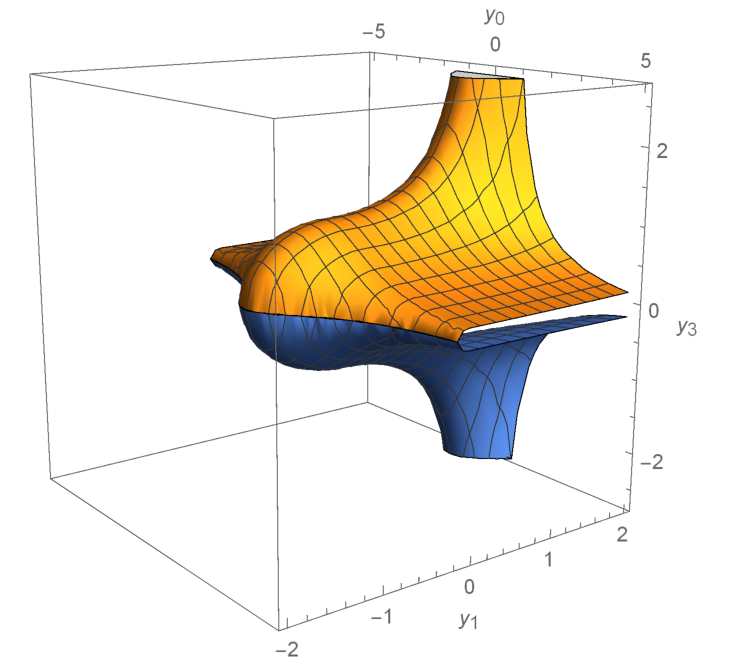
\includegraphics[width=0.562\linewidth]{Hole_with_matter_embedding.pdf}
	\caption{\label{pic_emb}The section $y^4 = y^5 = 0$ in the coordinates $ y^0 $, $ y^1 $ and $ y^3 $.}
\end{figure}

\bibliographystyle{my3beznazv}
\bibliography{paston-grav-e}
\end{document}